\documentclass[11pt]{article}
%بسم الله الرحمن الرحیم

%You should edit DSLecture.tex, not this file!
\usepackage{amsthm}
\usepackage{latexsym}
\usepackage{amssymb}
\usepackage{verbatim}
\usepackage{enumitem,amsmath,array}
\usepackage{tikz}
\usepackage{tkz-graph}
\usepackage{bookmark}
\usetikzlibrary{positioning,chains,fit,shapes,calc}
\usepackage[a4paper, margin=0.7in]{geometry}
\usepackage{listings}
\usepackage{clrscode3e}
\usepackage{hyperref}
\hypersetup{
	colorlinks=true,
	linkcolor=blue,
	filecolor=magenta,      
	urlcolor=cyan,
}
\usepackage[fontsloadable]{xepersian}


\settextfont[ExternalLocation=HM XNiloofar font/]{HM_XNiloofar}
\setdigitfont[ExternalLocation=HM XNiloofar font/]{HM_XNiloofar}
%\setdigitfont{ParsiDigits}
\defpersianfont\outline[Scale=1, ExternalLocation=HM XNiloofar font/]{HM_XNiloofarOl}

\setlength{\parindent}{1.5em}
\setlength{\parskip}{0.9em}
\renewcommand{\baselinestretch}{1.4}


\newcommand{\lecture}[3]{
%\pagestyle{empty}
{
	\begin{center}
			\vspace{-1cm}
		   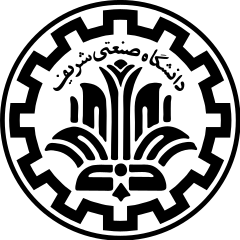
\includegraphics[scale=0.15]{Sharif}%\hfill \\[1em]  
	\end{center}
	\vspace{-8mm}
\begin{center}

\bf
%\begin{outline} 
{
\Large
ساختمان داده‌ها (۲۲۸۲۲)
}
%\end{outline} 
\\
مدرس: مرتضی علیمی
\\~
[پاییز $98$]
\end{center}
}\vspace*{-1em}
\noindent
جلسه #1: #2 \hfill نگارنده: #3
\vspace{-4mm}
\rule{\textwidth}{1pt}
\ \\
}

% example environment
\newenvironment{example}
{\smallskip \noindent \emph{مثال:}}
{\hfill $\boxtimes$ \smallskip}


\newtheorem{theorem}{قضیه}
\newtheorem{proposition}{گزاره}
\newtheorem{claim}{ادعا}
\newtheorem{lemma}{لم}
\newtheorem{corollary}{نتیجه}
\newtheorem{definition}{تعریف} % Use this for non-trivial definitions.

 %%%%%%%%%%%%%%%%%%%%%%%%%%%%%%%%%%%%%%%%%%%%%%%%%%%%%%%%%%%%%%%%%%%%%%%%%%%%


\usepackage{clrscode3e}

\begin{document}
\lecture{  }{درخت \lr{kd}}{مهرسا پوریا}
درخت \lr{kd}
\LTRfootnote{kd Tree}
داده ساختاری برای نگهداری نقاط در فضای 
\lr{k}
بعدی است. هر نقطه در فضای \lr{k}
بعدی را میتوان توسط \lr{k}
مولفه به صورت 
$x = (x_1, x_2, \cdots, x_k)$
نمایش داد. 
پیشتر با درخت جست و جوی دودویی آشنا شدیم که برای نگهداری اعداد حقیقی مناسب بود. حال اگر اعداد \lr{k}
بعدی باشند میتوان از درخت \lr{kd}
که در هر عمق درخت روی یک بعد مشابه درخت جست و جوی دودویی است استفاده کرد.
در ادامه با ساختار این درخت آشنا شده و چند پرسش
\LTRfootnote{Query}
که این ساختمان داده قابل به پاسخ گویی به آن است را بررسی خواهیم کرد.
\section{آشنایی با درخت \lr{kd}}
در درخت جست و جوی دودویی کلید هر گره محور اعداد حقیقی را به دو قسمت تقسیم میکرد، حال اگر این ایده را به ابعاد بالاتر تعمیم دهیم، میخواهیم هنگامی که کلید یک گره 
\lr{k}
بعدی باشند فضای \lr{$R^k$}
را متناظر با آن کلید به دو قسمت تقسیم کنیم؛ برای اینکار به یک ابر صفحه 
\lr{$k-1$}
بعدی
نیاز داریم.
راه های مختلفی برای اینکار وجود دارد اما ساده ترین ایده میتواند این باشد که برای هر گره متناظر با عمقش یک ابر صفحه انتخاب کنیم که خط عمود بر آن موازی محور مختصات متناظر با بعد منتسب به آن عمق باشد و با تغییر عمق گره به صورت متناوب بعد منتسب به هر عمق را عوض کنیم.
به بعدی که به هر گره نسبت میدهیم، بعد برش دهنده 
\LTRfootnote{Cutting Dimension}
میگوییم.
به علاوه هر گره صرفا زیرفضایی را افراز میکند که گره های با ارتفاع بالاتر آن محدود کرده اند. (به فضای محدود شده ای که هر گره در آن قرار میگیرد سلول آن گره 
\LTRfootnote{cell}
میگوییم.)
این خاصیت این گونه به دست می آید که در هر گره با توجه به بعد برش دهنده
(\lr{cd})
آن مقایسه رخ می دهد و نقاطی که مولفه \lr{cd}
کمتری از مولفه \lr{cd}
ام کلید گره
دارند در سمت چپ آن و در غیر این صورت در سمت راست آن گره قرار میگیرند. 
در ادامه یک مثال از \lr{2dTree}
و تقسیم فضای دوبعدی توسط آن میبینیم.
برای ساخت درخت برای یک مجموعه اعداد داده شده میتوانیم برای متوازن شدن درخت ساخته شده در هر مرحله به گونه ای فضا را برش بزنیم که تعداد داده های دو طرف تقریبا برابر باشد که این معادل انتخاب میانه از بین اعداد سلول با توجه به بعد برش دهنده است. 
\\
\begin{example}
فرض کنید نقاط زیر را داریم :
\begin{align*}
    (35,40),(50,10),(60,75),(80,65), (85,15) , (5, 45), (25,35), (90, 5)
\end{align*}
    در این صورت درخت نشان داده شده در شکل 1، یک 
    \lr{2d Tree}
    معتبر روی این نقاط است. همانگونه که در شکل مشخص شده است در ریشه مقایسه بر اساس بعد اول
    (\lr{x})
    صورت میگیرد و در عمق بعدی مقایسه بر اساس بعد دوم 
    (\lr{y})
    صورت میگیرد. همچنین در این شکل تقسیم فضای دو بعدی توسط خطوط متناظر با هر گره را میبینیم.
\begin{figure}[h]
    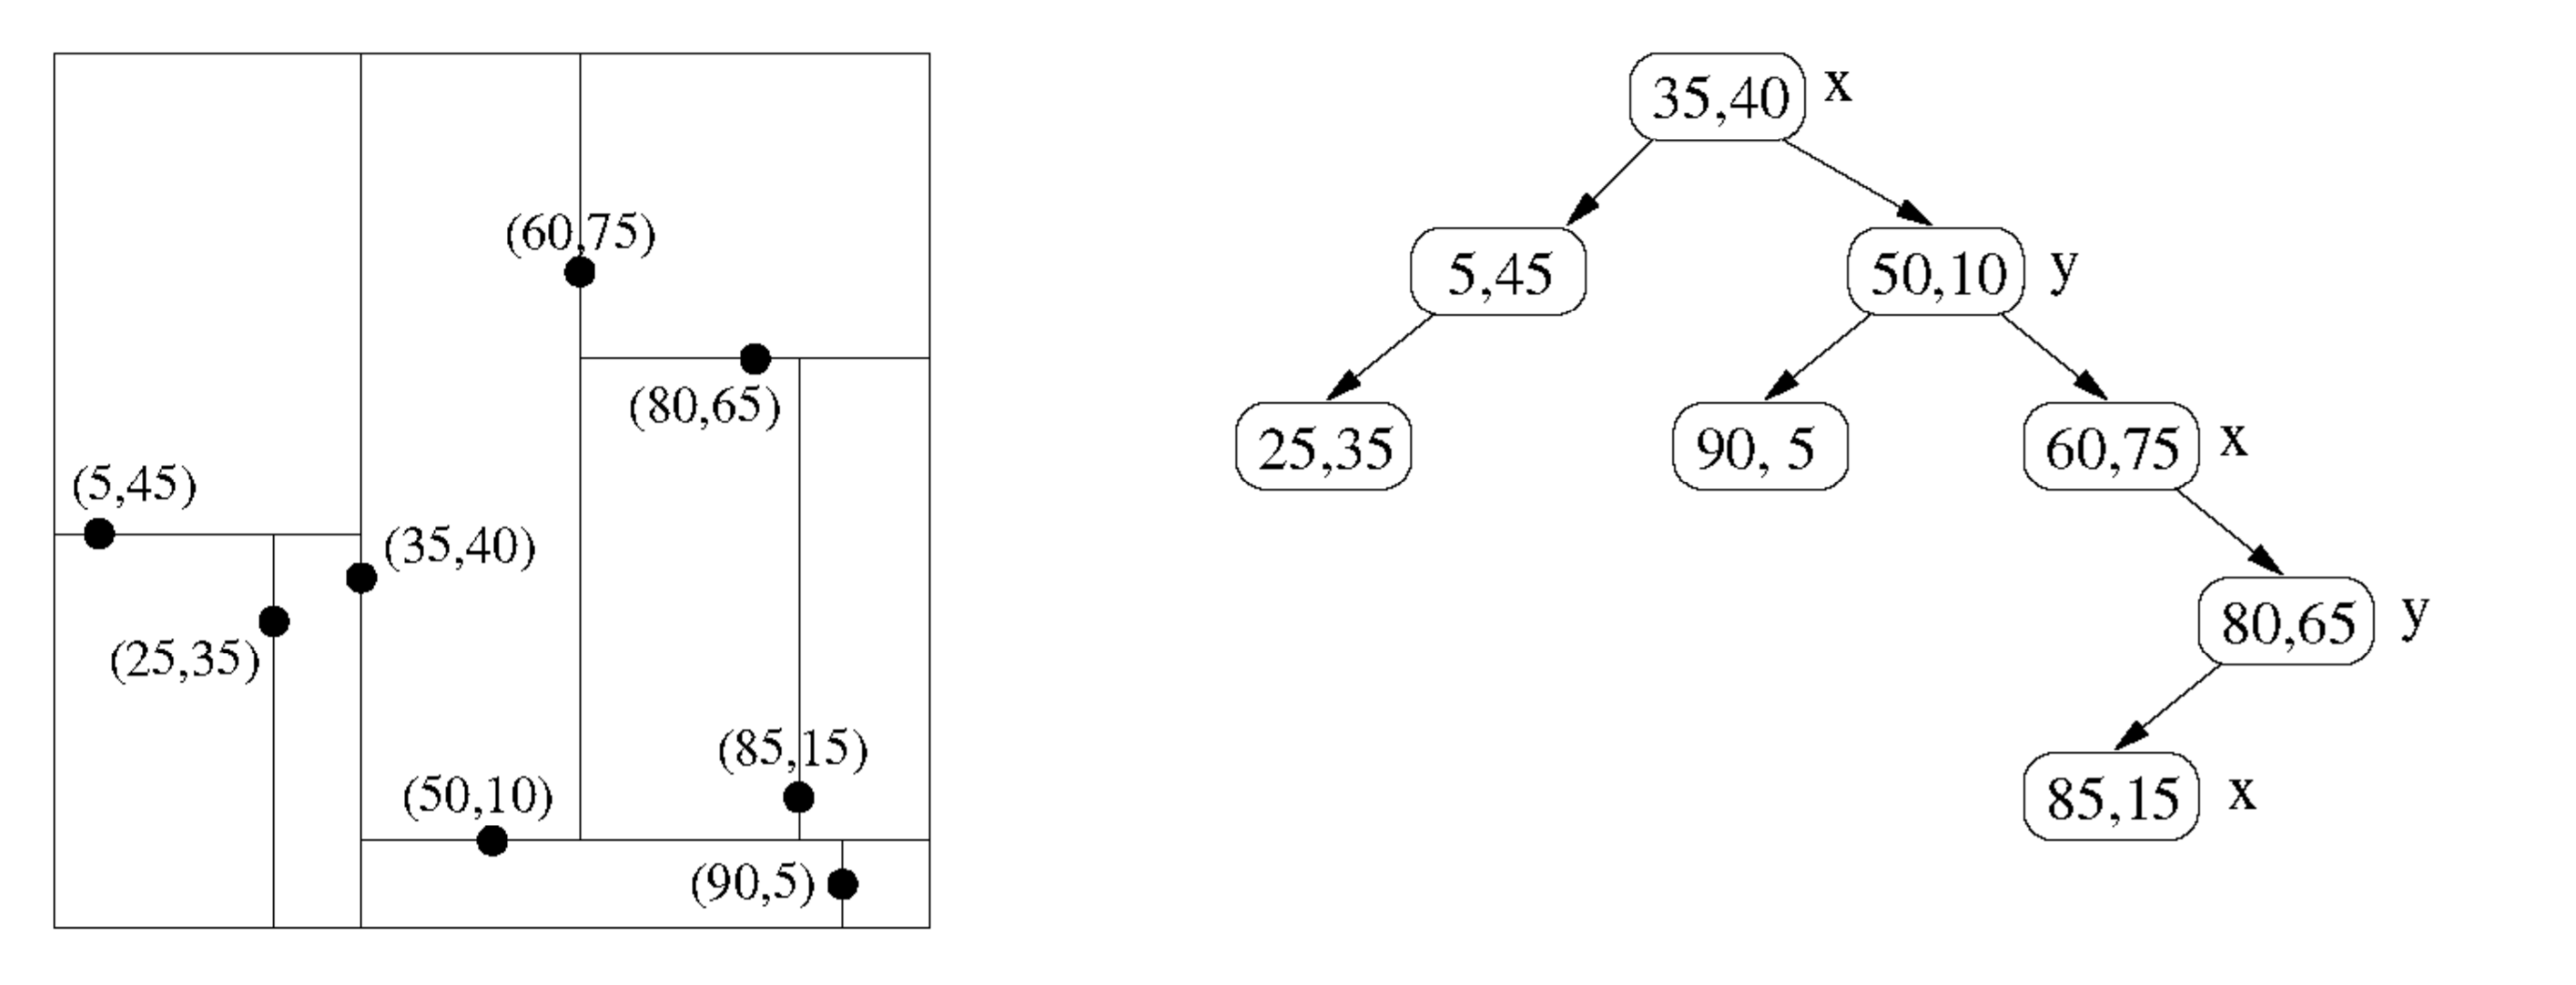
\includegraphics[scale=0.5]{fig1.PNG}
    \caption{\lr{2d Tree}}
    \centering
\end{figure}
\end{example} 
\section{اضافه کردن}
فرض کنیم یک درخت 
\lr{kd}
معتبر با ریشه
\lr{$root$}
داریم. میخواهیم نقطه 
\lr{$x$}
را به درخت اضافه کنیم، برای اینکار تابع 
\lr{$INSERT(x, root, 0)$}
را صدا میزنیم. این تابع مشابه درخت جست و جوی دویی در هر گره با توجه به بعد برش دهنده اش 
\lr{$(cd)$}
مقایسه را انجام میدهید و در صورتی که مولفه 
\lr{$cd$}
ام 
\lr{$x$}
از مولفه 
\lr{$cd$}
ام کلید گره کوچکتر باشد آن را در سمت چپ گره و در غیر این صورت در سمت راست آن اضافه میکند و با هر بار حرکت روی درخت بعد برش دهنده را متناوبا با توجه به ساختار درخت تغییر میدهیم. در این جا فرض شده که ابعاد برش دهنده نسبت داده شده به هر گره با توجه به عمق آن و به صورت متناوب از 
\lr{$0$}
تا 
\lr{$Dim-1$}
است.
مرتبه زمانی اضافه کردن گره از مرتبه 
\lr{$O(h)$}
است که 
\lr{$h$}
عمق درخت است و در صورتی که درخت متوازن باشد 
از مرتبه 
\lr{$O(log \ n)$}
است. 
\begin{latin}
\begin{codebox}
\Procname{$\proc{insert}(node \ x, KDNode \ t, int \ cd)$}
\li \If $(t == null)$ 
\li \Do $t = new \quad KDNode(x)$
\li
\Else \If ($x[cd] < t.data[cd]$)
\li $t.left = insert(x, t.left, (cd+1) \mod Dim)$
\li \Else 
\li $t.right = insert(x, t.right, (cd+1) \mod Dim)$
\End
\li \Return
\end{codebox}
\end{latin}
\section{یافتن کمینه در یک بعد}
برای یافتن کمینه یک بعد 
\lr{$(dim)$}
اگر در یک گره بعد برش دهنده برابر 
\lr{$dim$}
باشد فقط جست و جو را در زیر درخت سمت چپ آن گره ادامه میدهیم و در غیر این صورت باید هر دو زیر درخت سمت چپ و راست آن گره را جست و جو کنیم.
یافتن بیشینه نیز به همین صورت و با تغییرات جزئی انجام میشود. 
یافتن کمینه مشابه درخت جست و جوی دودویی در حذف درخت استفاده میشود. 
\begin{latin}
\begin{codebox}
\Procname{$\proc{findMin}(node \ T, int \ dim, int \  cd)$}
\li \If $(T == null)$ 
\li \Do \Return $null$
\End
\li \If ($cd == dim$)
\li \Do \If $(T.left == null)$ \Return $t.data$
\li \Do \Else \Return $findMin(T.left, dim, (cd+1) \mod Dim)$
\End
\li \Else
\li  \Return $minimum($
\li \Do $findMin(T.left, dim, (cd+1) \mod Dim),$
\li  $findMin(T.left, dim, (cd+1) \mod Dim),$
\li  $T.data$
\li $)$
\End
\end{codebox}
\end{latin}
\section{یافتن نزدیک ترین همسایه}
یکی از مهمترین \lr{query}
ها که توسط 
\lr{kd tree}
میتوانیم به آن پاسخ دهیم یافتن نزدیک ترین همسایه به یک نقطه در فضاست. پاسخ به این پرسش کاربردهای زیادی از جمله در الگوریتم های یادگیری ماشین مانند
\lr{KNN} \LTRfootnote{K nearest neighbours}
دارد.
فرض کنیم مجموعه نقاط 
\lr{S}
در یک درخت 
\lr{kd}
ذخیره شده است. 
میخواهیم نقطه ای از 
\lr{S}
که کمترین فاصله با نقطه ورودی 
\lr{$Q$}
را دارد بیابیم.
فرض کنیم نزدیکی را بر اساس کم بودن فاصله اقلیدسی بین نقاط تعریف کنیم.
فرض کنید که در ابتدا حدسی برای نزدیکترین نقطه 
\lr{$(best)$}
داریم. 
اگر فرض کنیم نقاط دو بعدی هستند
 اگر نقاط نزدیک تر به این نقطه وجود داشته باشد باید در داخل دایره به مرکز \lr{q}
و شعاع اندازه فاصله بین   \lr{q}
و نقطه حدس زده شده 
\lr{$(bestDist)$}
می افتند.
در فضای \lr{$d$}
بعدی در داخل کره \lr{$d$}
بعدی می افتد که به آن ابرکره نامزد
\LTRfootnote{Candidate hypersphere}
میگوییم.
این مشاهده از آنجا اهمیت دارد که توسط آن
میتوانیم
بخش هایی از درخت که مطمئنیم جواب نزدیکترین همسایه در آن نیست را حذف کنیم.
به این کار هرس کردن 
\LTRfootnote{Pruning}
گفته میشود. 
حال به استفاده از این شهود به توضیح الگوریتم 
\lr{$NN$}
می پردازیم.
در ابتدا
\lr{$best = null$}
و 
\lr{$bestDist =\infty$}
می باشد. 
\lr{cd}
همان بعد برش دهنده است که در قسمت های قبل به آن اشاره کردیم و 
و 
\lr{$BB$}
سلول آن گره است. این پارامتر از این جهت اهمیت دارد که اگر فاصله ی همه ی نقاط داخل یک محدوده از 
\lr{$Q$}
بیشتر از بهترین فاصله فعلی بود دیگر نباید آن محدوده را جست و جو کنیم. 
وقتی وارد گره 
\lr{$T$}
میشویم اول تعیین میکنیم که سلول مربوط به آن آیا میتواند جوابی بهتر از بهترین جواب فعلی تولید کند یا خیر اگر نه از آن گره خارج میشویم. سپس اگر خود گره فاصله کمتر از 
\lr{$bestDist$}
داشت مقادیر مربوط به جواب را با مقدار خود گره به روز رسانی میکنیم. در نهایت به جست و جو در زیر درخت های آن گره میپردازیم در ابتدا باید بررسی کنیم که در کدام سمت ابر صفحه مربوط به آن گره قرار داریم اگر در سمت چپ قرار داشتیم ابتدا سلول سمت چپ و سپس سلول سمت راست و در غیر این صورت برعکس عمل میکنیم. این کار در واقع برای این است که بخش هایی که احتمالا جواب بهینه در آن قرار دارد را زودتر بررسی کنیم. 
فرض میکنیم توابع 
\lr{$trimLeft$}
و 
\lr{$trimRight$}
سلول مربوط به چپ و راست را بر میگردانند. 
اگر بخواهیم مرتبه ی زمانی این الگوریتم را بررسی کنیم در بدترین حالت هر گره یکبار بازدید میشود مرتبه زمانی جست و جوی نزدیک ترین همسایه از 
\lr{$O(n)$}
است. 
اما میتوان نشان داد به
\lr{$O(2^k + log\ n)$}
نزدیک تر است، شهود آن این است که برای هر نقطه انتظار داریم همسایه های سلول مربوط به آن را در فضا بررسی کنیم که تعداد آنها 
\lr{$2^k$}
است و زمان 
\lr{$O(log n)$}
برای پایین آمدن در درخت و یافتن این گره ها نیاز داریم.
\begin{latin}
\begin{codebox}
\Procname{$\proc{NN}(node \ Q, kdTree \ T, int \ cd, Rect \ BB)$}
\li \If $(T == null)$ \Return 
\li \If $(distance(Q, BB) >= bestDist)$
\li \Do \Return 
\End
\li $(dist = distance(Q, T.data))$
\li \If $dist < bestDist$
\li \Do $best = T.data$
\li $bestDist = dist$
\End
\li \If $(Q[cd] < T.data[cd])$
\li \Do $NN(Q, T.left, nextCd, BB.trimLeft(cd, t.data))$
\li $NN(Q, T.right, nextCd, BB.trimRight(cd, t.data))$
\li $f$
\Else 
\li $NN(Q, T.right, nextCd, BB.trimRight(cd, t.data))$
\li $NN(Q, T.left, nextCd, BB.trimLeft(cd, t.data))$
\End
\End
\End
\end{codebox}
\end{latin}

\bibliographystyle{alpha}

\begin{thebibliography}{99}
	\begin{latin}	%english reference
		
		%book in MLA style: https://owl.purdue.edu/owl/research_and_citation/mla_style/mla_formatting_and_style_guide/mla_works_cited_page_books.html
		\bibitem{q}
		https://www.cs.umd.edu/users/meesh/420/ContentBook/FormalNotes/MountNotes/lecture17-quadkd.pdf.
		\bibitem{2}
		https://www.cs.umd.edu/users/meesh/420/ContentBook/FormalNotes/MountNotes/lecture18-kd2.pdf
		\bibitem{3}
		http://stanford.edu/class/archive/cs/cs106l/cs106l.1162/handouts/assignment-3-kdtree.pdf
	\end{latin}	
\end{thebibliography}
\end{document}
